% !TeX spellcheck = en_US


\chapter{Infrastructure}

\subsection{Service Descriptions and Data Flow}

The overall system is composed of several interconnected services, as illustrated in \cref{fig:data_flow}.
Below, we provide a description of each service and its role within the system:

\begin{itemize}
    \item \textbf{Sensor IO Module:}
    This microcontroller reads sensor data from the robot's I2C buses.
    It is responsible for publishing the collected sensor data to the MQTT Broker and for forwarding control commands from the controller to the actuator.

    \item \textbf{Controller:}
    The Controller processes sensor data and generates control signals.
    It also publishes statistics for further monitoring.

    \item \textbf{MQTT Broker:}
    Acting as the central messaging hub, the MQTT Broker receives and distributes sensor and control data.
    It is based on the subscriber-publisher model.
    This real-time data exchange is critical for system responsiveness.

    \item \textbf{Telegraf:}
    Telegraf collects sensor data and controller performance metrics.
    The data is then forwarded to InfluxDB for storage.

    \item \textbf{InfluxDB:}
    InfluxDB is a time-series database that stores historical sensor data and controller performance metrics.
    This data is used for trend analysis and performance monitoring over time.

    \item \textbf{Grafana:}
    Grafana provides a web-based dashboard that visualizes the sensor data in real-time.
    It allows users to monitor the system's status interactively.

    \item \textbf{Promtail:}
    Promtail is responsible for collecting logs from the various services and forwarding them to Loki.
    This facilitates centralized logging and aids in debugging.

    \item \textbf{Loki:}
    Loki aggregates the logs provided by Promtail and makes them available for visualization via Grafana.
    This centralized logging system helps in troubleshooting and monitoring system health.

    \item \textbf{Traefik:}
    Traefik is used as a reverse proxy to route external HTTP requests to appropriate services (such as Grafana and the MQTT Broker).
    It simplifies access control and ensures that services are securely exposed.
\end{itemize}

\noindent The data flow in the system is summarized in the following Mermaid diagram:

\begin{figure}[H]
    \centering
    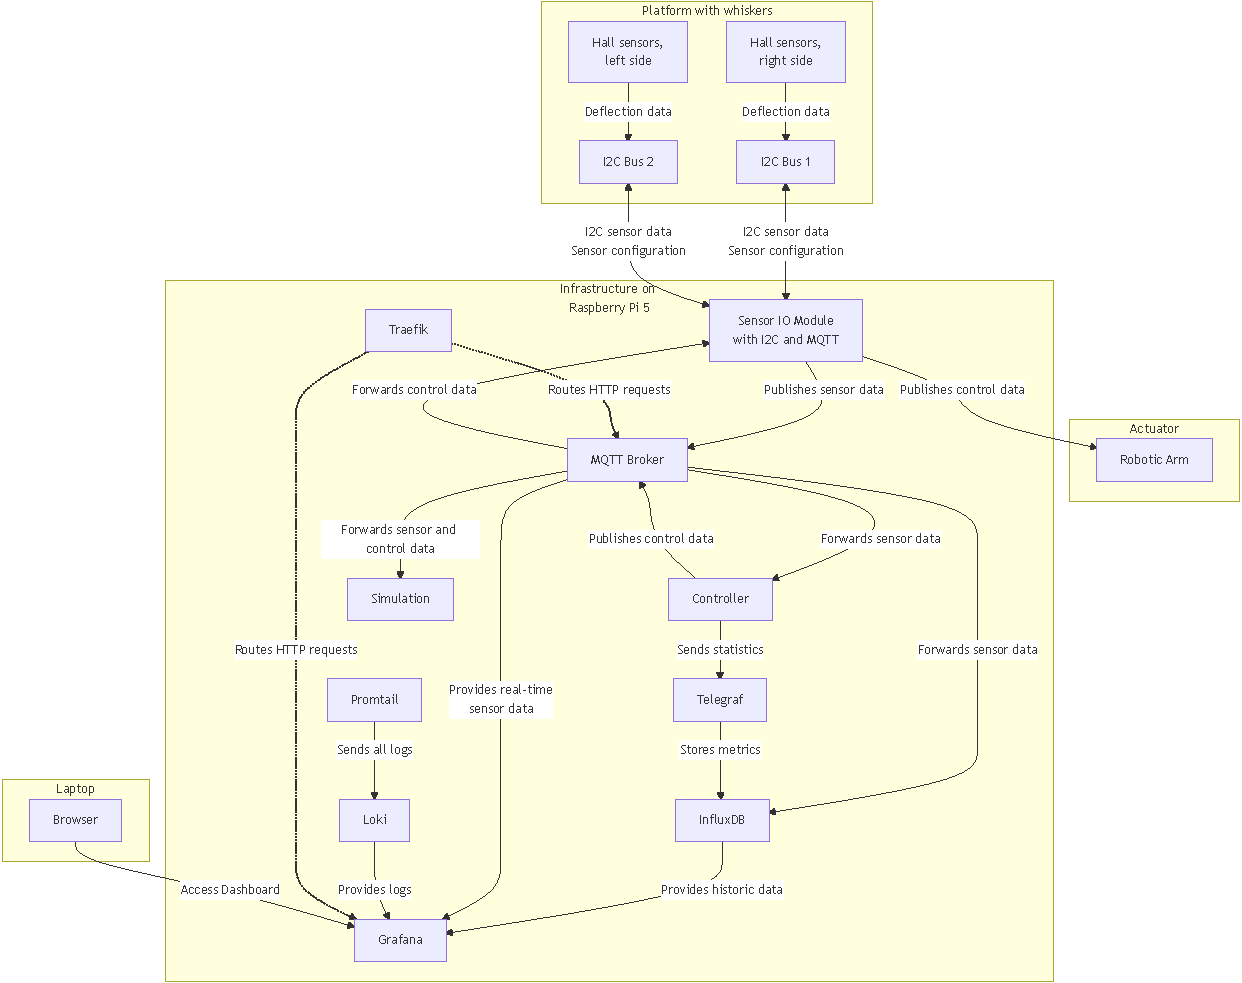
\includegraphics[width=\textwidth]{figures/services}
    \caption{Data flow in the system infrastructure.}
    \label{fig:data_flow}
\end{figure}


\subsection{MLX90393 Sensor Drivers}
Two MLX90393 sensor drivers were implemented: one for the ESP32 microcontroller in C++ and another for the Raspberry Pi in Python.
Both provide an API to read sensor data and configure the sensor's settings.
